\titre{Tail Symbols}
%%%%%%%%%%%%%%%%%%%%%%%%%%%%%%%%%%%%%%%%%%%%%%%%%%%%%%%%%%%%%%%%%%%%%%%%%%%%%%

% Un aide-m�moire des symboles math�matiques est disponible en ligne:
% http://auteurs.h-k.fr/annales/Doc/aide-memoire/symboles-mathematiques.pdf


\question{The (current ?) definition}
Quoting the paper: 'we call tail symbol the 
symbol that follows the last symbol inserted in the DST'.
What I'm wondering is if the tail symbol is picked from
\begin{itemize}
  \item the same sequence that generated the phrase that was 
        just inserted into the DST
  \item or the beginning of the sequence that follows this phrase ?
\end{itemize}

In the latter case, I'm considering the same example as in 
the paper : the parsing of the eight sequences (these are only their inserted prefixes) :
\centers{$1 \quad 10 \quad 0 \quad 101 \quad 00 \quad 01 \quad 000 \quad 100$}


Is this figure then accurate about the tail symbols ? (I hope not
because this definition seems to contradict other things)
\centers{
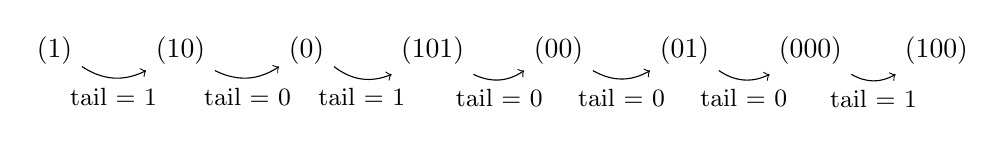
\begin{tikzpicture}[node distance=1.6cm]

% nodes
\node (A) at (0, 0) {(1)};
\node (B) [right of=A] {(10)};
\node (C) [right of=B] {(0)};
\node (D) [right of=C] {(101)};
\node (E) [right of=D] {(00)};
\node (F) [right of=E] {(01)};
\node (G) [right of=F] {(000)};
\node (H) [right of=G] {(100)};

% arrows
\path[->] (A) edge[bend right] node [below] {\small tail = 1} (B);
\path[->] (B) edge[bend right] node [below] {\small tail = 0} (C);
\path[->] (C) edge[bend right] node [below] {\small tail = 1} (D);
\path[->] (D) edge[bend right] node [below] {\small tail = 0} (E);
\path[->] (E) edge[bend right] node [below] {\small tail = 0} (F);
\path[->] (F) edge[bend right] node [below] {\small tail = 0} (G);
\path[->] (G) edge[bend right] node [below] {\small tail = 1} (H);

\end{tikzpicture}}
% Pas de \end{document} ici: voir 'main.tex

Using this definition
  \begin{itemize}
    \item 0 occurs four times as the tail symbol
    \item 1 occurs three times
  \end{itemize}
  
Therefore, in the last paragraph before equation $(1)$, 
${T_8}^{(0)}$ should be $4$ rather than $5$ ? 
And we could now define the tail symbols as \emph{the first
symbol of each sequence except the first one} ? 

But then it seems to clash
with the definition of $T_n = (T_n^a, T_n^b)$, having
$T_n^a$ as the number of times 'a' appears as a tail symbol assuming that
\emph{all} sequences start with symbol 'a'. If \emph{all} means 'all the $n$ sequences'
then the tail symbols definition is absurd because all the tail symbols 
are just 'a' ?

As for the recursion 
\centers{$ T_{n+1}^a = \delta_a + T_{n_a}^a + T_{n_b}^b $}

$\delta_a$ is "equal to 1 when the second symbol of the first sequence is 'a'"
suggests that we should use all the first sequence and not only its prefix 
that is being inserted in the DST ?

Another final problem with this 
definition is that I don't see the probabilistic value of the first
symbol of each independent sequence : I could actually initialize them with any value,
although I'd probably use the stationary distribution to pick that first symbol.

\question{The (right ?) definition}
Therefore I think right now that the definition of the tail symbols
would rather be, since we are in the 
Markov Independent model : if a phrase 
\centers{$ p = w_1 \dots w_n $} is inserted from a sequence 
\centers{$ X = w_1 \dots w_n \,w_{n+1} \dots$}
then the tail symbol of that phrase is $w_{n+1}$. 
Therefore, to define the tail symbols, for example for $n=4$, with the sequences
$X(1) = 00000\dots$, $X(2) = 1010101\dots$, $X(3) = 1001101\dots$ and
$X(4) = 001100111\dots$, which give the parsing 
  \centers{$()(0)(1)(10)(00)$}
we would do, 
with the \textcolor{red}{prefix phrases} in red and the \textcolor{green}{tail symbol} in green :

\begin{egalites}
  & X(1) 
    & {\color{red}{0}} {\color{green}{0}} 00000\dots \\
  &X(2) 
    & {\color{red}{1}} {\color{green}{0}}10101\dots \\
  & X(3) 
    & {\color{red}{10}} {\color{green}{0}} 1101 \dots \\
  & X(4) 
    & {\color{red}{00}} {\color{green}{1}} 100111\dots
\end{egalites}

This means that the tail symbols are not obvious from the DST, 
and this reconciles with the definition of $\delta_a$. If this is the 
correct definition, then the tree of figure 1 is misleading because
we need the sequences to define the tail symbols. (as well as 
the phrase 'in Figure 1 the tail symbol after phrase (10) is "0")






